\chapter{THIẾT KẾ MẠCH VÀ GIAO DIỆN ĐIỀU KHIỂN}

\section{Sơ đồ khối}
    Sơ đồ khối thiết kế bộ điều khiển được mô tả trên \fig{\ref{Fig:block-diagram}}:

    \begin{figure}[htp]
        \begin{center}
            %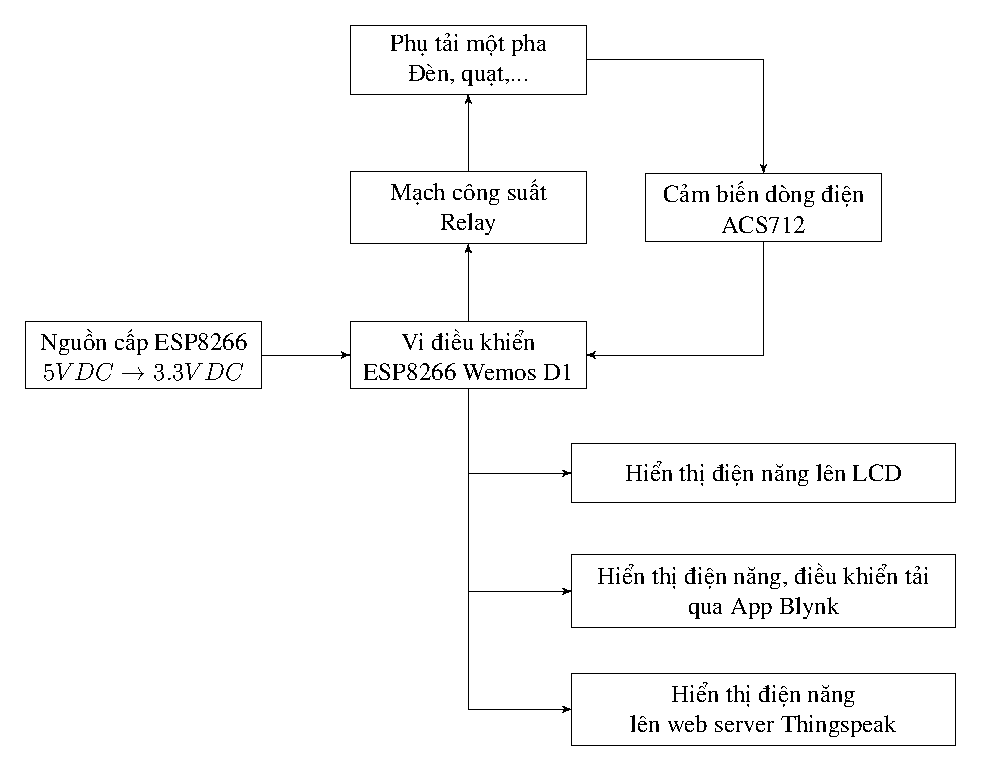
\includegraphics[scale=1]{block-diagram.pdf}
            \subimport{../flowchart/}{block-diagram.tex}
        \end{center}
        \caption{Sơ đồ khối thiết kế bộ điều khiển} \label{Fig:block-diagram}
    \end{figure}

    Mô tả các khối chức năng trên \fig{\ref{Fig:block-diagram}}:
    \begin{itemize}
        \item Sử dụng vi điều khiển ESP8266 Wemos D1 với khả năng giao tiếp WiFi (với nguồn hoạt động 5VDC $\rightarrow$ 3.3VDC).
        \item Điều khiển tải thông qua mạch công suất với Relay (sử dụng nguồn kích 5VDC).
        \item Sử dụng cảm biến dòng điện ACS712 để đo dòng điện tiêu thụ của phụ tải xoay chiều một pha, từ đó tính công suất, điện năng tiêu thụ của phụ tải.
        \item Hiển thị, gửi dữ liệu thu thập được (dòng điện, công suất) lên LCD (quan sát trực tiếp), App Blynk (quan sát trên thiết bị di động) và Server Thingspeak (quan sát trên Web).
    \end{itemize}

\section{Sơ đồ mạch nguyên lý}
    Sơ đồ mạch nguyên lý được mô tả trên \fig{\ref{Fig:powerACS712_schem}}:
        \begin{figure}[htp]
            \begin{center}
                \fbox{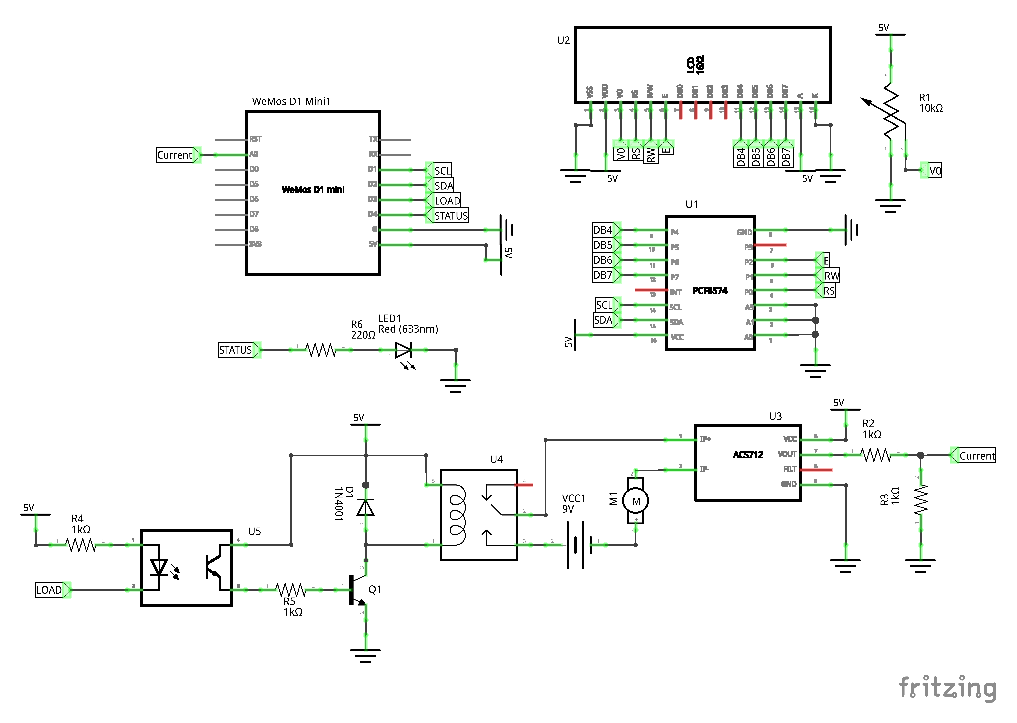
\includegraphics[scale=.85]{powerACS712_schem.pdf}}
            \end{center}
            \caption{Sơ đồ mạch nguyên lý} \label{Fig:powerACS712_schem}
        \end{figure}

\section{Mô tả các khối chức năng trên sơ đồ mạch nguyên lý}
    \begin{itemize}
        \item Hiển thị dòng điện và công suất với LCD 16x02 (sử dụng giao tiếp I2C).
        \item Đo dòng điện tiêu thụ của phụ tải với cảm biến dòng ACS712.
            \begin{itemize}
                \item Do tín hiệu điện áp đưa vào chân analog của ESP8266 Wemos D1 tối đa là 3.3V, trong khi đó tính hiệu trả về của cảm biến có thể lên đến 5.0V.
                \item Sử dụng cầu chia điện áp tại ngõ ra của cảm biến dòng để điện áp đưa vào chân analog của ESP8266 nhỏ hơn 3.3V. Do $R_2 = R_3 = R = 1 k \Omega$, nên:
                    \begin{align*}
                        V_o = \dfrac{R}{R + R} V_i = \dfrac{V_i}{2} \Longrightarrow V_i = 2.0 V_o
                    \end{align*}
                \item Khi đó các công thức tính dòng điện được xác định lại như sau:
                    \begin{itemize}
                        \item Với dòng DC:
                            \begin{align*}
                                V_{(mV)} & = \dfrac{2.0 \times adc \times 5000.0}{1024.0} = \dfrac{adc \times 5000.0}{521.0};\\ I_{(mA)} & = \dfrac{V - 2500}{V_m} \quad \textrm{(với } V_m \textrm{ là độ nhạy)}
                            \end{align*}
                        \item Với dòng AC:
                            \begin{align*}
                                V_{(mV)} & = \dfrac{2.0 \times adc_{MaxPoint} \times 5000.0}{1024.0} = \dfrac{adc_{MaxPoint} \times 5000.0}{512.0};\\ I_{(mA)} & = \dfrac{V - 2500}{\sqrt{2}V_m} \quad \textrm{(với } V_m \textrm{ là độ nhạy)}
                            \end{align*}
                    \end{itemize}
            \end{itemize}
        \item Điều khiển tải thông qua relay.
        \item LED báo trạng thái quá tải.
    \end{itemize}

\section{Giao diện điều khiển trên Blynk}
    \begin{figure}[htp]
        \begin{center}
            \fbox{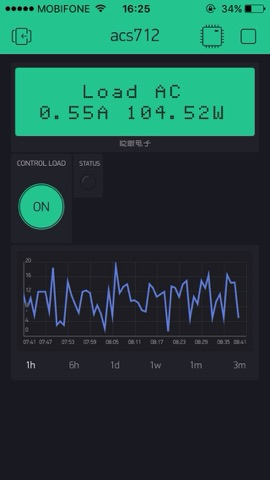
\includegraphics[scale=.5]{blynk-result}}
        \end{center}
        \caption{Giao diện điều khiển trên Blynk}
    \end{figure}

    \begin{table}[htp]
        \begin{center}
            \begin{tabular}{|l|c|l|} \hline
                \textbf{Phần tử} & \textbf{Pin} & \textbf{Giải thích} \\
                \hline
                LCD & V0 & Hiển thị dữ liệu \\
                \hline
                Button & D5 & Điều khiển tải \\
                \hline
                LED & V1 & Báo trạng thái quá tải \\
                \hline
                History Graph & V3/V4 & Dữ liệu dòng điện DC/AC\\
                \hline
            \end{tabular}
        \end{center}
        \caption{Các phần tử trên App Blynk}
    \end{table}

\newpage
\section{Giao diện thu thập dữ liệu trên Thingspeak}
    \begin{table}[htp]
        \begin{center}
            \begin{tabular}{|c|l|} \hline
                \textbf{Tên Field} & \textbf{Giải thích} \\
                \hline
                Field 3 & Dòng DC \\
                \hline
                Field 4 & Trạng thái quá tải \\
                \hline
                Field 5 & Công suất tiêu thụ \\
                \hline
            \end{tabular}
        \end{center}
        \caption{Các Field trên web Thingspeak}
    \end{table}
